\section{Численные эксперименты}
\label{sec:Chapter4} \index{Chapter4}

% \subsection{Тест 1}
\par Тесты производились на интересующей нас задаче – линейной системе с многими 
правыми частями, возникающей при решении задачи электромагнитного рассеяния 
методом интегральных уравнений \cite{stavtsev2009application}. Порядок системы - 14144, количество правых частей - 722.
Каждая правая часть соответствует разным углам падения, а также первая половина правых частей отличается от второй типом поляризации. 
При этом матрица системы является комплексной и симметричной.
\begin{figure}[H] 
    \begin{subfigure}{.5\textwidth}
        \centering
        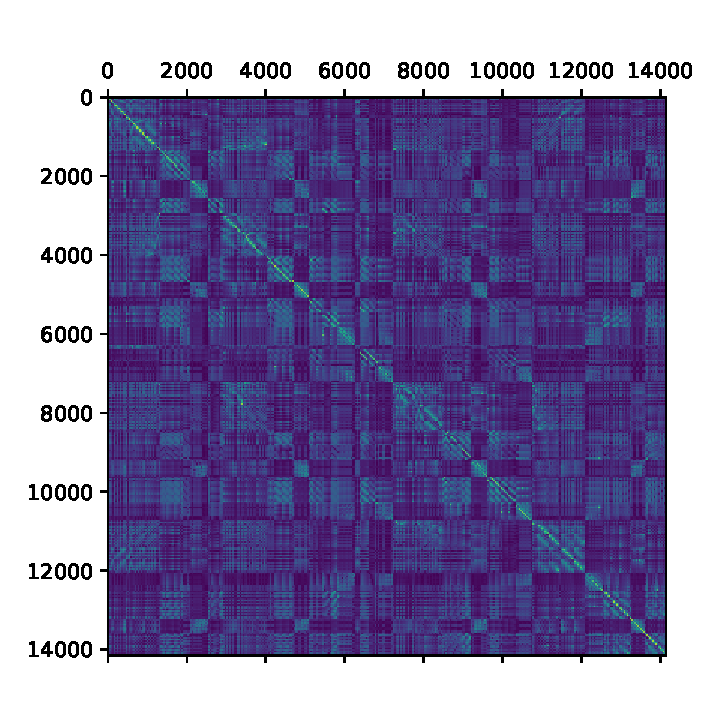
\includegraphics[width=0.7\linewidth]{images/mat.pdf}
        \caption{Матрица системы в логарифмическом масштабе (отображены модули элементов матрицы).}
        \label{fig:matrix}
    \end{subfigure}
    \begin{subfigure}{.5\textwidth}
        \centering
        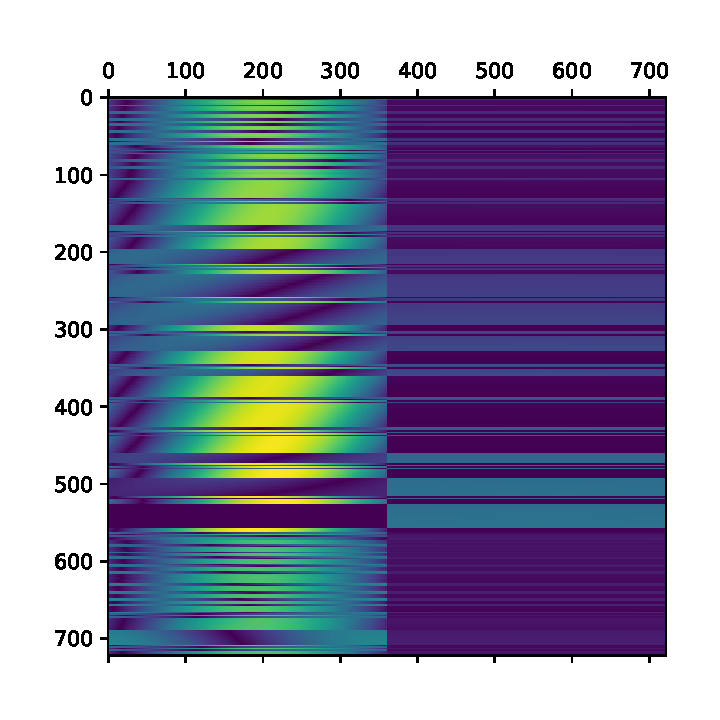
\includegraphics[width=0.7\linewidth]{images/rhs.pdf}
        \caption{первые 722 строки блока правых частей в логарифмическом масштабе (отображены модули элементов матрицы).}
        \label{fig:rhs}
    \end{subfigure}
    \caption{}
    \label{fig:matrixnrhs}
\end{figure} 
 На рис.\ref{fig:matrixnrhs} представлен вид матрицы системы и первые 722 строки блока
 правых частей. Из-за разных поляризаций первая половина правых частей сильно отличается от второй половины, и 
 если применять блочные крыловские алгоритмы к блоку правых частей, содержащему правые части из первой и второй половины
 одновременно, то алгоритмы могут очень плохо себя показывать в таком сценарии.

\begin{figure}[H]
    \centering
    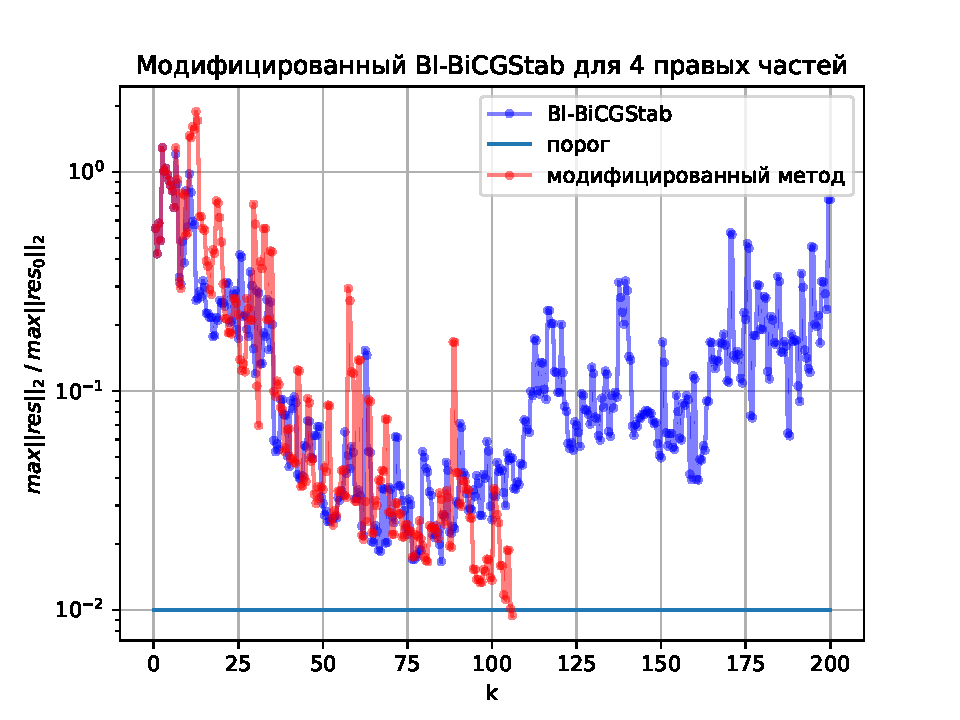
\includegraphics[width=0.7\linewidth]{images/4.pdf}
    \caption{}
    \label{fig:4}
\end{figure} 
\par Первый тест демонстрирует, что метод из статьи \cite{elGuennouni2003} не достигает требуемой точности, в то время как 
версия с улучшениями, описанными в главе \ref{sec:Chapter3}, сходится. 
Эксперимент проводился в одинарной точности для четырех правых частей с номерами: 0, 90, 180, 270. Его результаты представлены
на рис.\ref{fig:4}
% \subsection{Тест 2}
\begin{figure}[H]
    \centering
    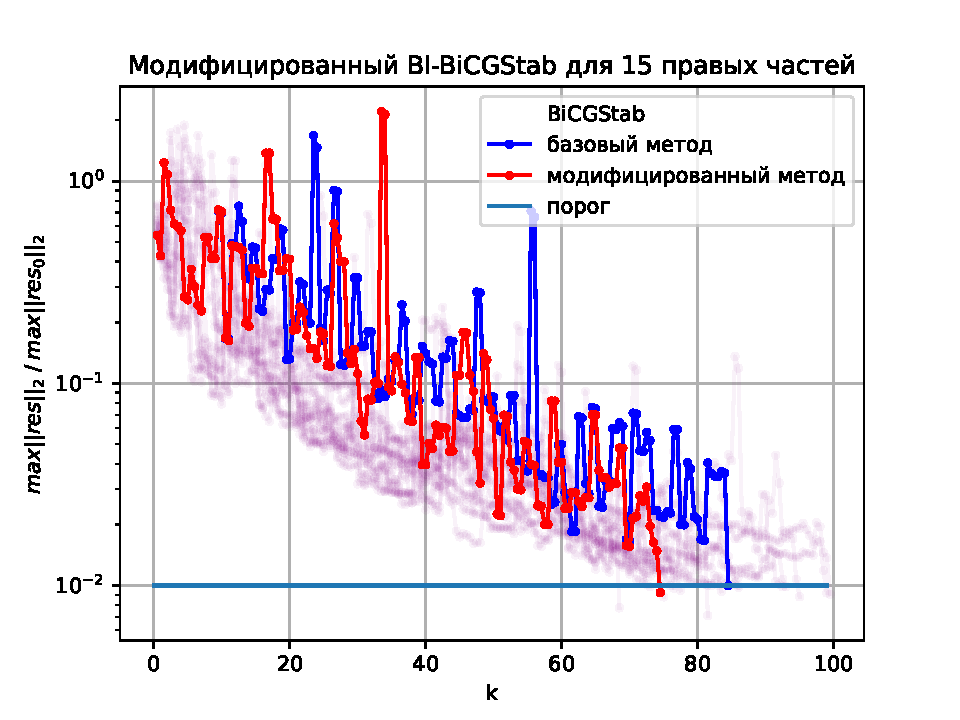
\includegraphics[width=0.7\linewidth]{images/acceleration_15_rhs.pdf}
    \caption{}
    \label{fig:acceleration_15}
\end{figure}
% \par 15 правых частей, уменьшения числа итераций, считаем в двойной точности
\par Второй тест демонстрирует, что улучшения, описанные в главе \ref{sec:Chapter3} позволяют получить выгоду по количеству умножений матрицы системы на вектор,
по сравнению с решением систем с каждой правой частью в отдельности. Эксперимент проводился в двойной точности с 15 правыми частями,
выбранными с помощью RRQR. Его результаты представлены на рис.\ref{fig:acceleration_15}. По оси абсцисс - количество итераций, по оси
ординат - относительная максимальная невязка в блоке. Фиолетовым изображено падение невязки при решении задачи с каждой правой частью 
в отдельности, синим - метод из статьи \cite{elGuennouni2003}, красным - метод с улучшениями из главы \ref{sec:Chapter3}. Для решения этой задачи
стабилизированными бисопряженными градиентами было потрачено 2525 матрично-векторных умножений (МВУ), для решения методом из статьи \cite{elGuennouni2003} - 2535, модифицированный
метод сошелся за 2235 МВУ, таким образом выгода составил 12\% по сравнению с неблочной версией.
% \subsection{Тест 3}
% \par более 30 правых частей, демонстрация отсутствия взрыва невязки
% При количестве правых 
% \begin{figure}[H]
%     \centering
%     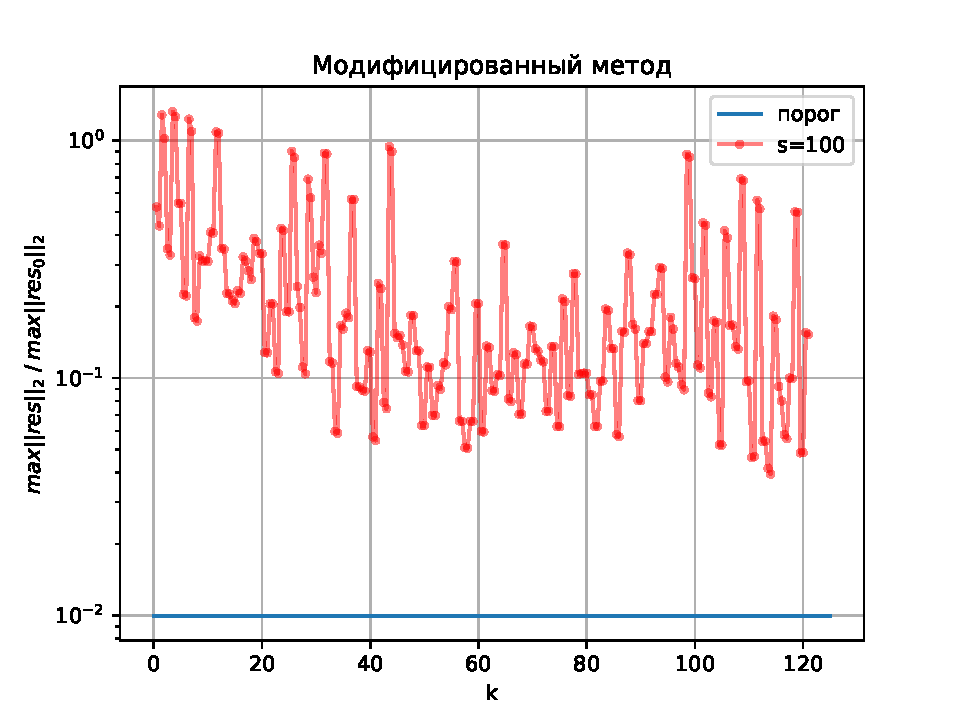
\includegraphics[width=0.7\linewidth]{images/100_rhs.pdf}
%     \caption{}
%     \label{fig:100_rhs}
% \end{figure}

\par Однако количество итераций даже при всех предложенных улучшениях все равно велико, так что
было принято решение рассмотреть алгоритм на основе метода квази-минимальных невязок, описанный 
в главе \ref{sec:bsqmr_mod}. 

\begin{figure}[H]
    \centering
    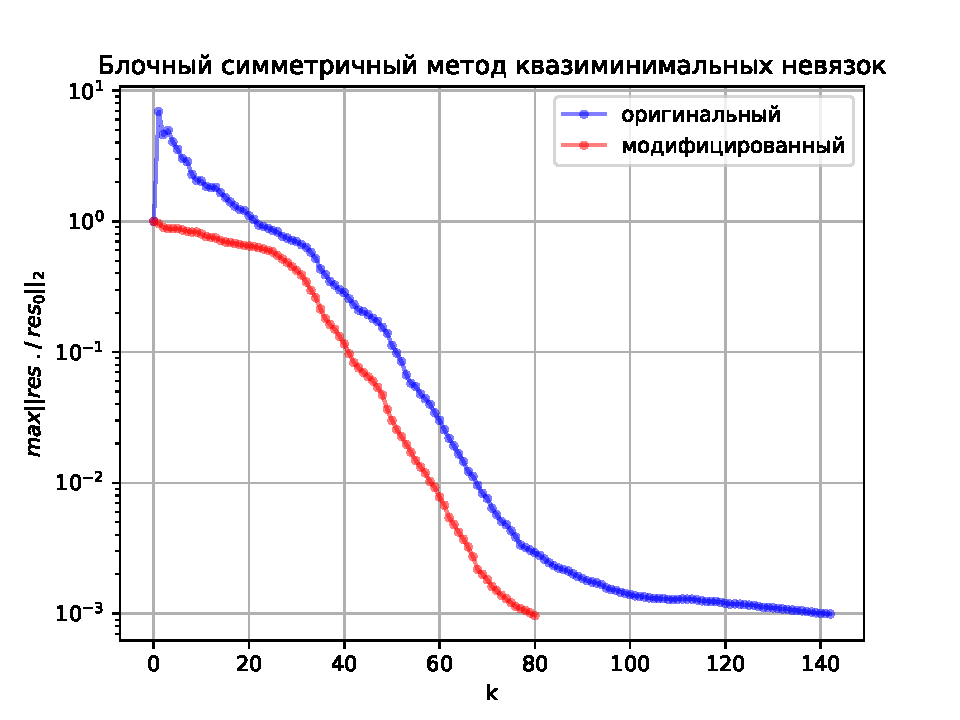
\includegraphics[width=0.7\linewidth]{images/bsqmr_reorth2_base_double_45.pdf}
    \caption{}
    \label{fig:bsqmr_reorth2_base_double_45}
\end{figure}

\par На рис.\ref{fig:bsqmr_reorth2_base_double_45} показано уменьшение максимальной
относительной невязки в блоке в зависимости от числа итераций, синяя кривая соответствует 
алгоритму из статьи \cite{doi:10.1137/0917019}, красная - модифицированному алгоритму из
главы \ref{sec:bsqmr_mod}. Эксперимент производился в двойной точности с 45 правыми частями, 
остановка происходила при достижении порога $10^{-3}$ для демонстрации различия в сходимости двух методов.
Примечательным моментом является скачок на первой итерации для метода из статьи \cite{doi:10.1137/0917019}, которого
нет в модифицированной версии по причинам, освещенным в конце главы \ref{sec:bsqmr_mod}.
%28,15,19

\begin{figure}[H]
    \centering
    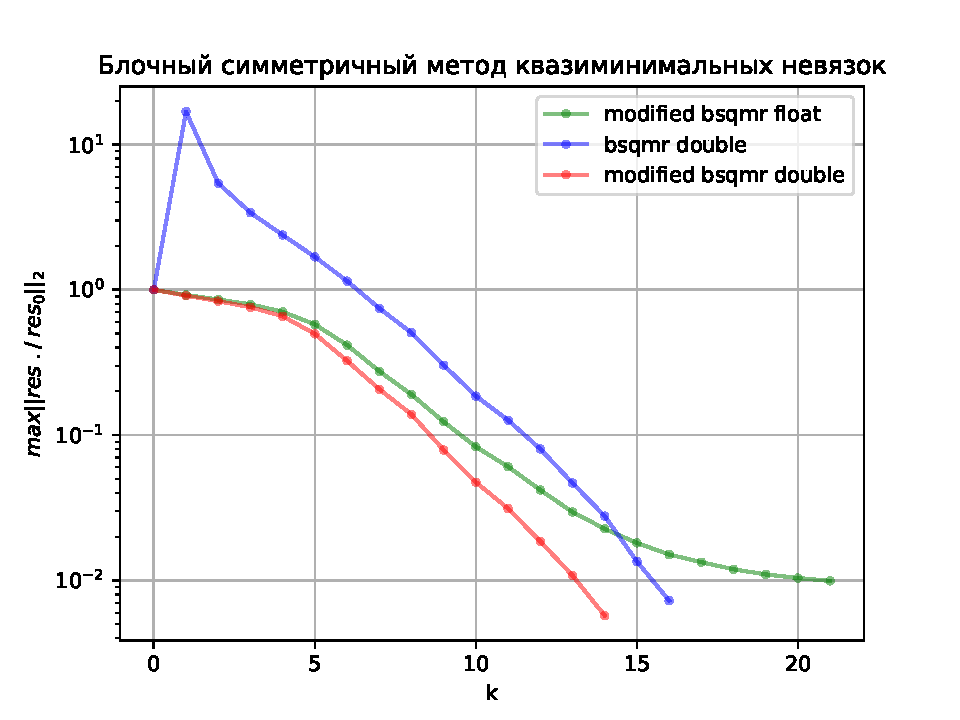
\includegraphics[width=0.7\linewidth]{images/bsqmr_722_base_reorth2_doublevsfloat.pdf}
    \caption{}
    \label{fig:bsqmr_722_base_reorth2_doublevsfloat}
\end{figure}

\par На рис.\ref{fig:bsqmr_722_base_reorth2_doublevsfloat} представлены результаты 
расчета со всеми 722 правыми частями одновременно. Синий график представляет алгоритм
из статьи \cite{doi:10.1137/0917019}, красный и зеленый графики - его модификацию из главы \ref{sec:bsqmr_mod}.
Причем расчёты для синей и красной кривых выполнены в арифметике с двойной точностью, а для зелёной - с одинарной.
Немодифицированный алгоритм в одинарной точности уже на первых итерациях показывает сильную расходимость,
поэтому эти расчёты не включены на график. 

\begin{figure}[H]
    \centering
    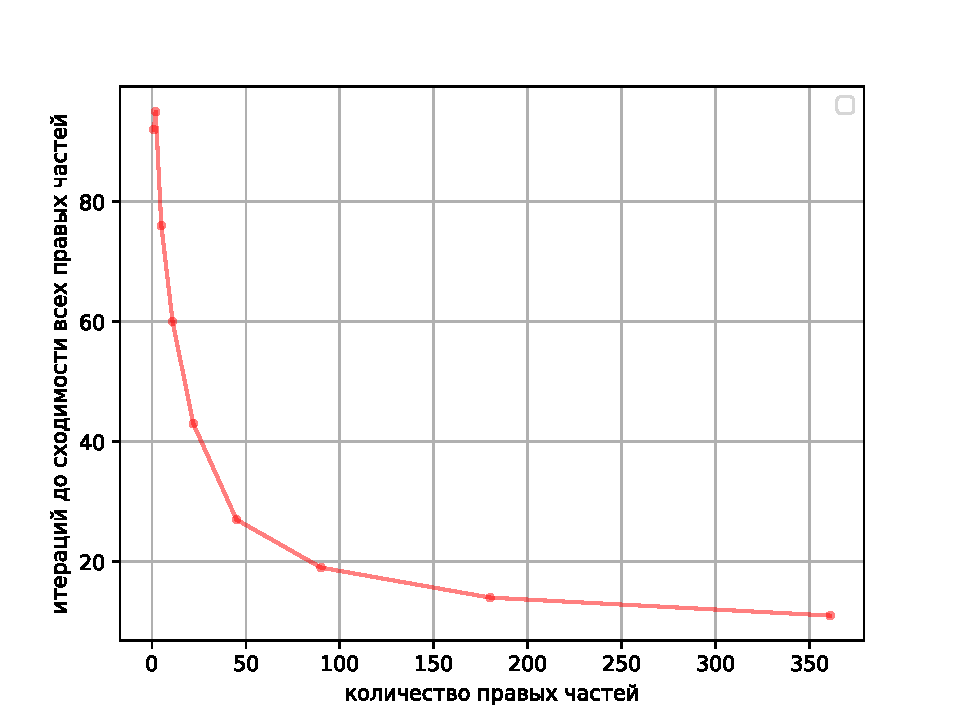
\includegraphics[width=0.7\linewidth]{images/mvss.pdf}
    \caption{Количество итераций модифицированного блочого симметричного метода квазиминимальных невязок в зависимости от количества задействованных правых частей}
    \label{fig:mvss}
\end{figure}

\par На рис.\ref{fig:mvss} изображена зависимость количества итераций блочого 
симметричного метода квазиминимальных невязок в зависимости от количества задействованных
 правых частей для первых 361 правой части в задаче электромагнитного рассеяния \cite{stavtsev2009application}.
Видно, что количество итераций уменьшается с увеличением размера блока, следовательно, уменьшается
и размер задействованного для решения крыловского пространства.   

\newpage
